\documentclass[14pt,landscape,color=UCLdarkred,margin=3cm]{uclposter}

\usepackage{amsmath,amssymb}
\usepackage{amsthm}
\usepackage{xcolor}
\usepackage{eso-pic}
\usepackage{authblk}
\usepackage{tikz}
\usepackage{environ}
\usepackage{graphicx}
\usepackage{float}
%\usepackage{physics}

\title{Scalable Quantum Simulation of Molecular Energies}

\author{James Mills}
\author{Shuhao Yang}
\author{Shanice St John}
\affil[1]{MSc Quantum Technologies, UCL}
% \affil[2]{TikZ, UCL}
% \affil[*]{a.example@ucl.ac.uk}

\begin{document}\large

\maketitle

\begin{multicols}{3}

\section*{Introduction}


Quantum computing is a rapidly advancing field predicted to revolutionise many
areas of science and technology. It is predicted to have important real-world applications in encryption and communication systems and in the development of new medicines and materials to name but a few. An important point is that these quantum computers are not considered a replacement to classical computers, they will only be brought to bear on certain types of problems which are too difficult for classical computers to solve. Classical computers is a term used to describe all everyday computational computing devices which rely on classical (non-quantum) phenomena to compute.

Simulating systems in quantum chemistry is a problem too difficult for classical computers. Efficient simulation of quantum chemistry experiments would enable a dramatic leap forward in our understanding of fundamental chemistry. For example it would significantly reduce the need for cumbersome and expensive trial-and-error techniques in the development of new medicines and materials.

\section*{Key terms}


\begin{highlightbox}[UCLdarkblue!20!white]
	\textbf{Qubit} For representation, we describe information as qubit in quantum mechanics. It is an analogous concept of the classical bit in which classical information is encoded in 0s and 1s. For the information stored in a qubit can be represented by a state.
\end{highlightbox}

\begin{highlightbox}[UCLstone!50!white]
  \textbf{Superposition} A qubit has extraordinary property, which can be in both states of `0' and `1' at the same time, but a classical bit is either `0' or `1'.
\end{highlightbox}



\begin{highlightbox}[UCLyellow!20!white]
\textbf{Quantum simulations in chemistry} Quantum theory is our best description of phenomena happening at the smallest scales imaginable. Simulating quantum systems with classical computers is extremely difficult, and becomes increasingly difficult as the size of the system increases. Quantum simulations with quantum computing hardware are much easier, as we are using quantum phenomena (the same phenomena that make the system difficult to describe with a classical computer) to boost our computing power.
\end{highlightbox}

\begin{highlightbox}[UCLmidgreen!20!white]
\textbf{Algorithm} A set of instructions used to solve a problem, especially by a computer. The instructions are created so that it can be understood by the computer. This is then sent to the quantum computer. The computer then follows the instructions using some program or software. The end of the process provides an answer or even many possible answers.
\end{highlightbox}

\columnbreak

\section*{Techniques in Paper}
The work by the researchers on the paper `Scalable Quantum Simulation of Molecular Energies' uses supercooled quantum qubits to run algorithms to find out information about the fundamental properties of molecules.
The variational quantum eigensolver (VQE) and the phase estimation algorithm (PEA) are two types of algorithm which are performed on supercooled qubit quantum computing hardware to output molecular energies. To use both algorithms, a special type of quantum hardware known as Superconducting Quantum Interference Devices (SQUIDs). This type of qubit has a superposition of ``charged" states and can be used in quantum circuits.

\begin{figure}[H]
  \begin{center}
%   \begin{minipage}[c]{15em}
  \begin{minipage}[c]{8em}
    % 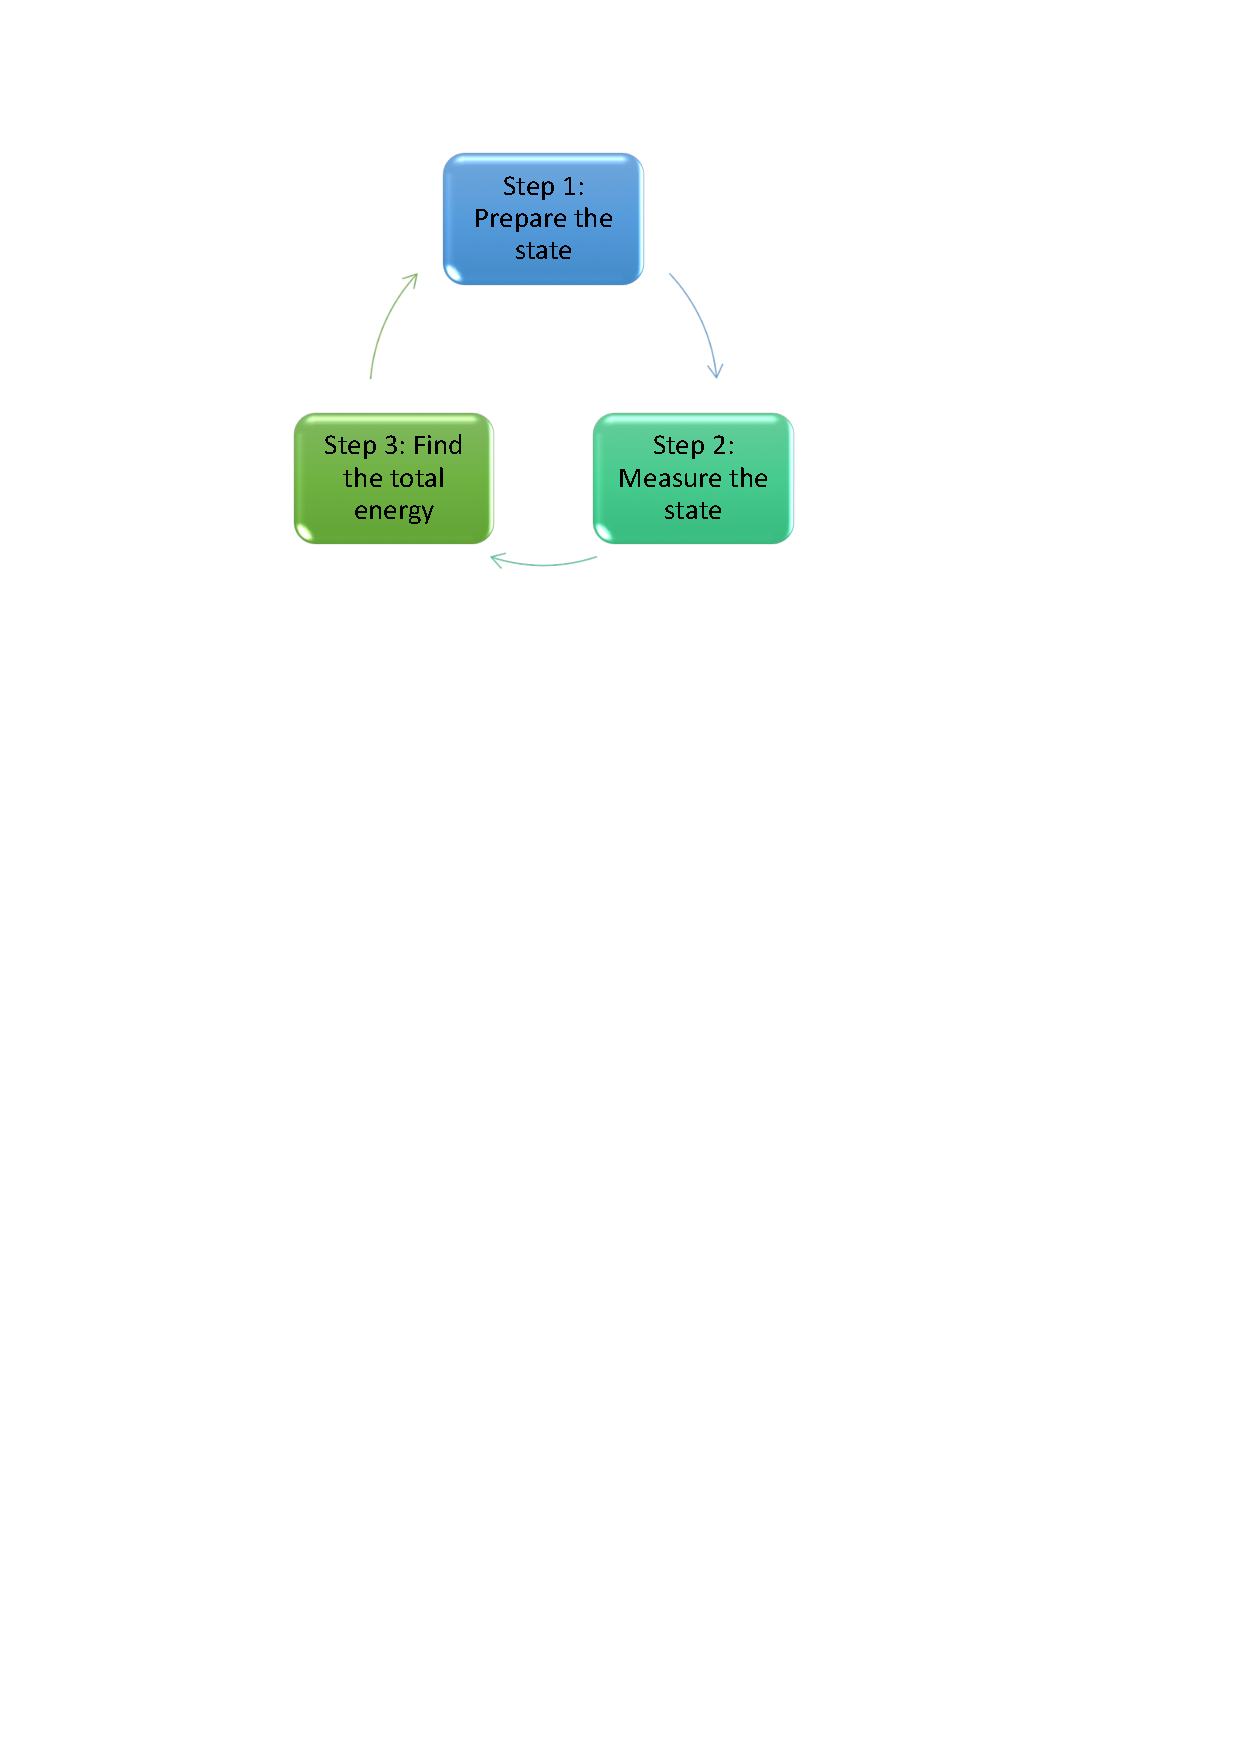
\includegraphics[width=15em]{VQEdiagram.pdf}
    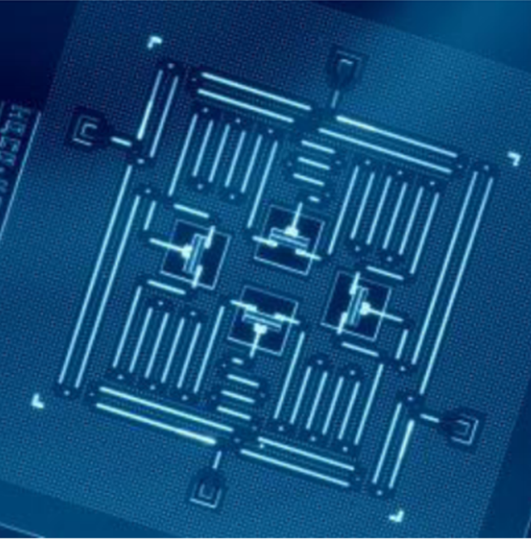
\includegraphics[width=8em]{4_Qubit.png}
  \end{minipage}
  \qquad
%   \begin{minipage}[c]{18em}
  \begin{minipage}[c]{20em}
    some words about hardware
  \end{minipage}
  \end{center}

   
\end{figure}




\subsection*{VQE}
\begin{highlightbox}[UCLpink!20!white]
  \begin{itemize}
\item Firstly, we start by preparing a state using a ``special" method. This method makes it possible for the algorithm run in the way that we want.
\item Secondly, we measure the total energy for each value of the distance. We must select the lowest value as we are focusing on the ground energy.
\item After that, a tool is then used to find more lower values of the total energy.
\item All steps are repeated until we reach the smallest value possible.
\end{itemize}
\end{highlightbox}

\subsection*{PEA}


PEA is the algorithm estimate the value of index over exponential coefficient in order to work out molecular energy.

\begin{highlightbox}[UCLpurple!20!white]
\begin{itemize}
\item Similarly to the VQE algorithm, we must prepare a state using another ``special" method since these are two different algorithms. 
\item Next, some ``magical" equipment must be set up in a superposition of states - this will make it possible to measure the state.
\item Then, we use some operations to set up the state and the apparatus so that it is ready to be measured. 
\item Finally, we measure the state to find the lowest value of the total energy. We repeat this process until find an accurate value of the total energy.
\end{itemize}
\end{highlightbox}



\begin{figure}[H]
  \begin{center}
%   \begin{minipage}[c]{15em}
  \begin{minipage}[c]{15em}
    % 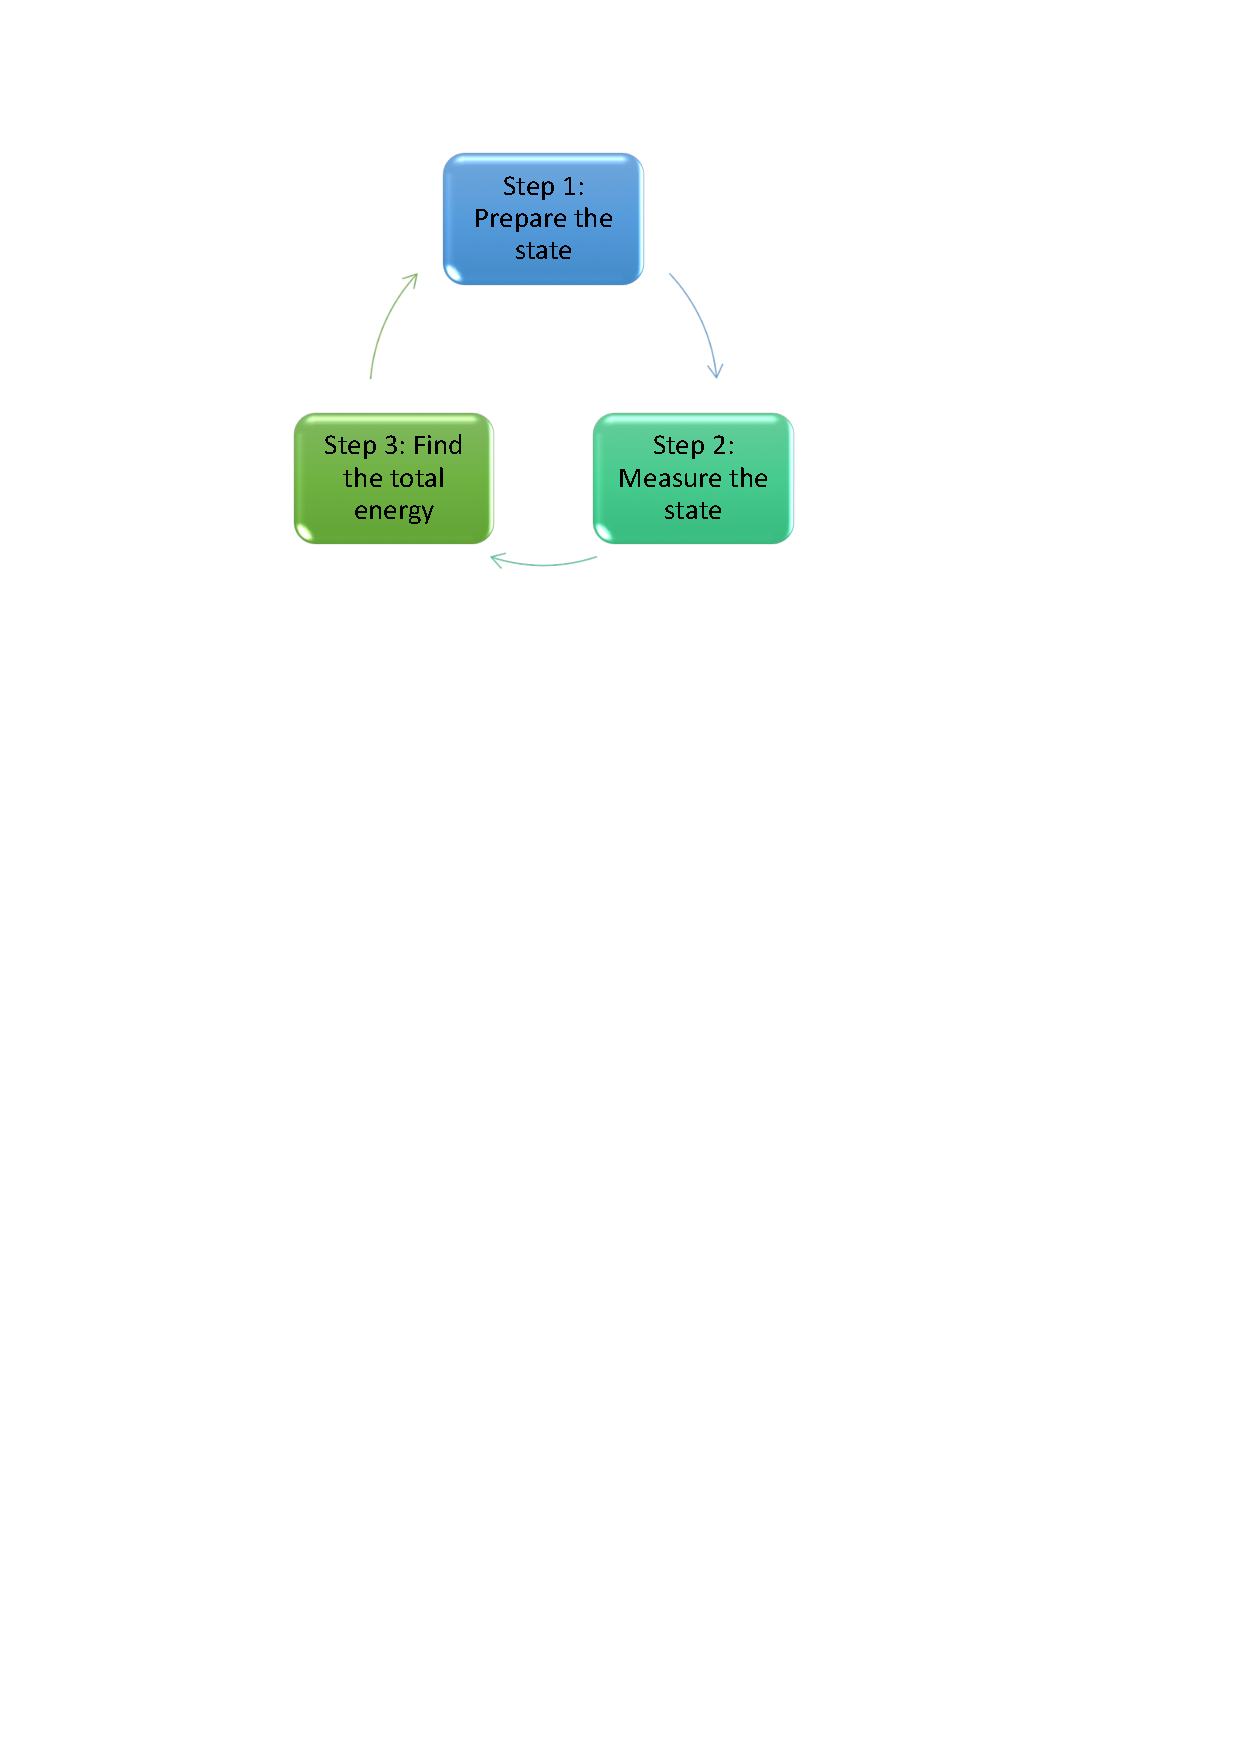
\includegraphics[width=15em]{VQEdiagram.pdf}
    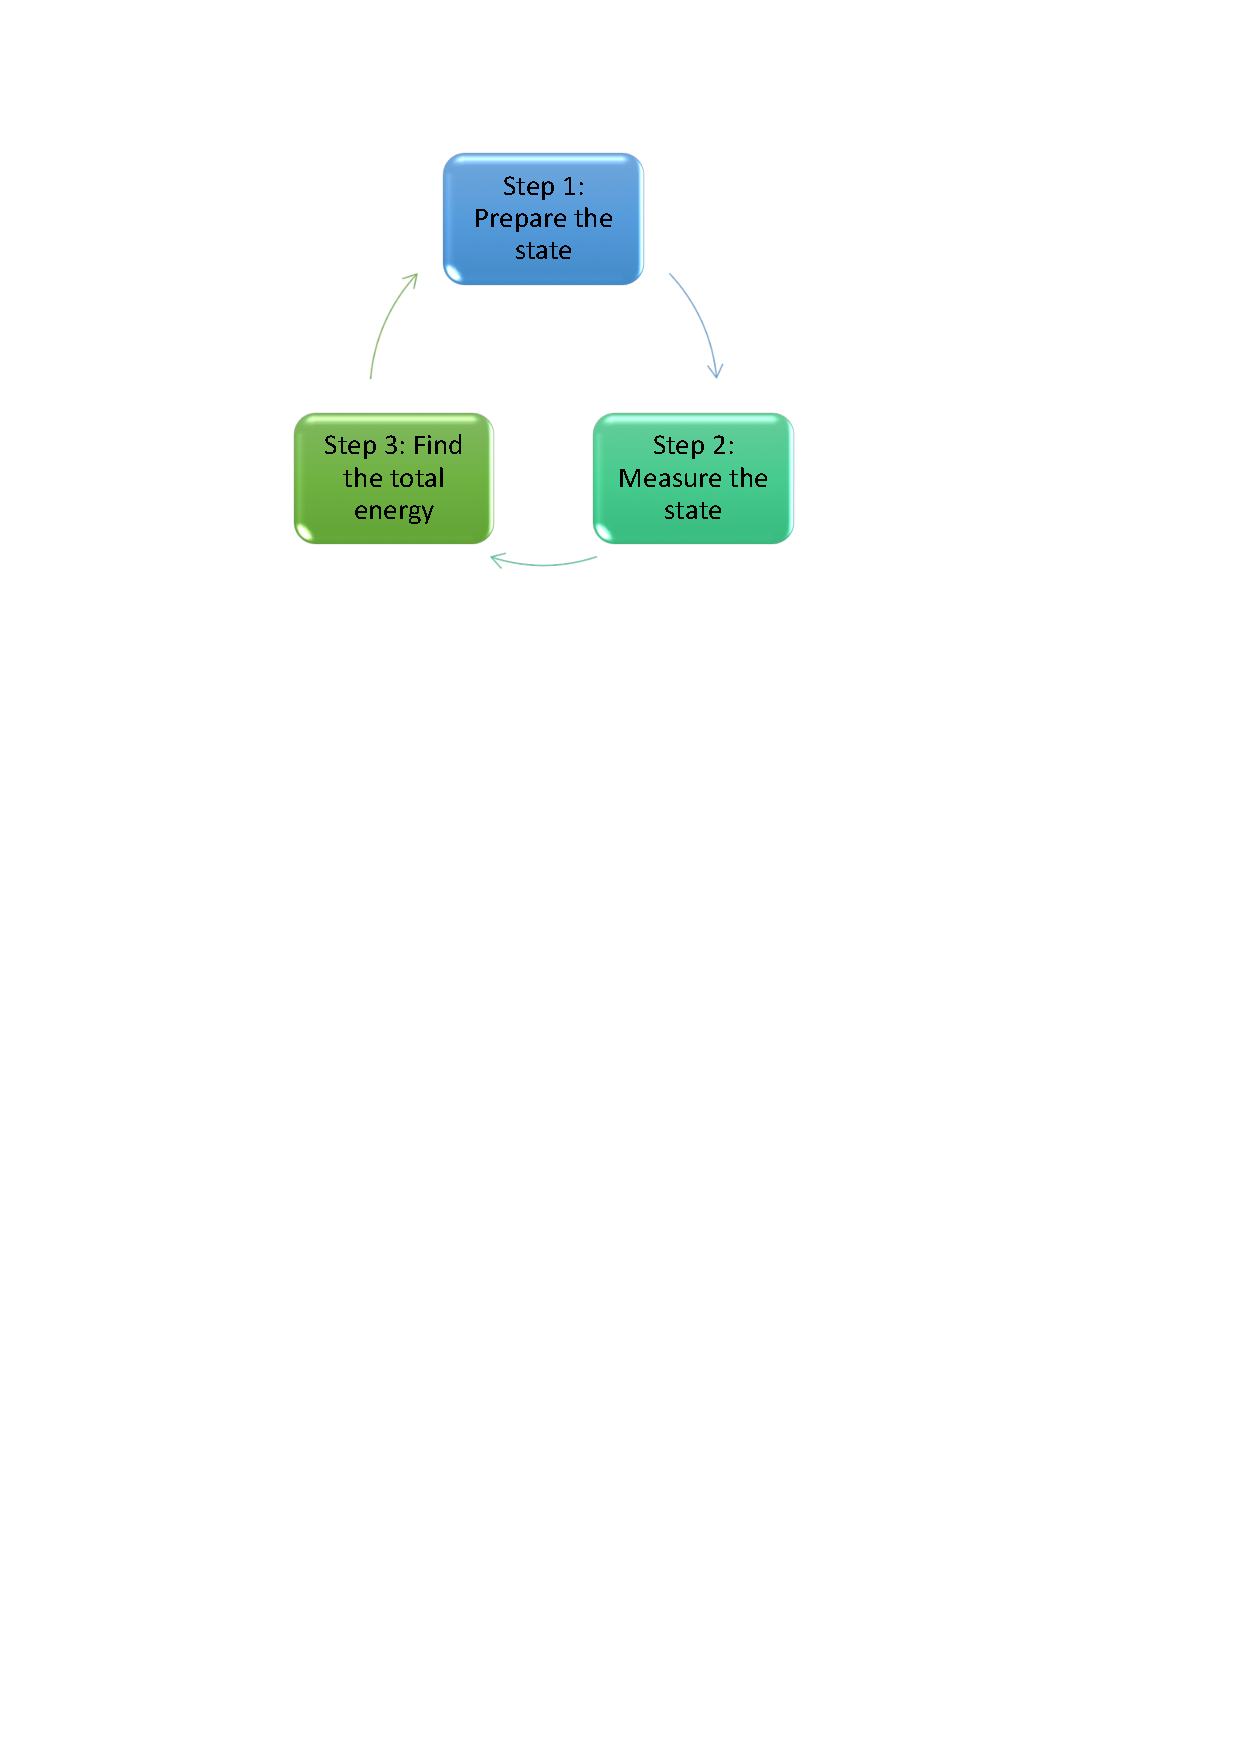
\includegraphics[width=15em]{VQEdiagram.pdf}
    \caption{VQE}
  \end{minipage}
  \qquad
%   \begin{minipage}[c]{18em}
  \begin{minipage}[c]{15em}
    % 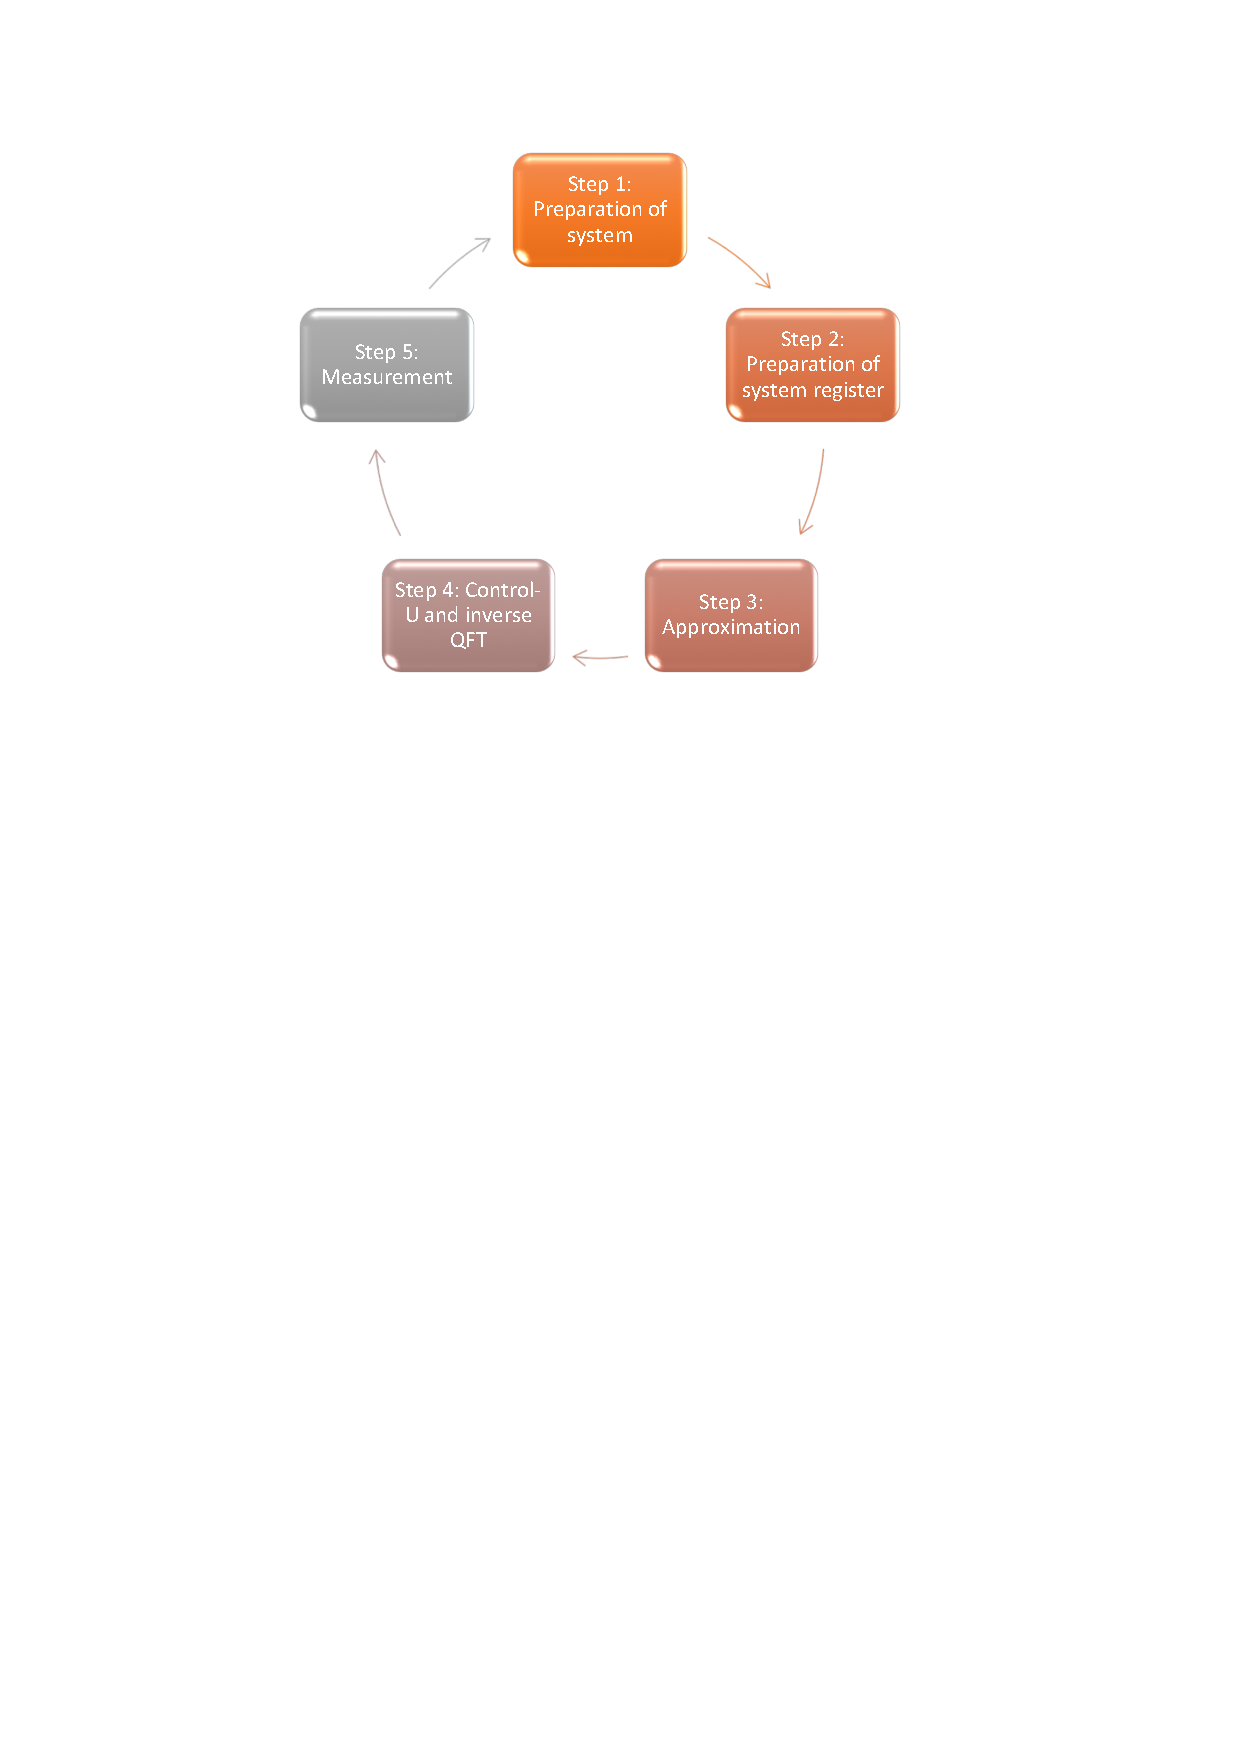
\includegraphics[width=18em]{PEA.pdf}
    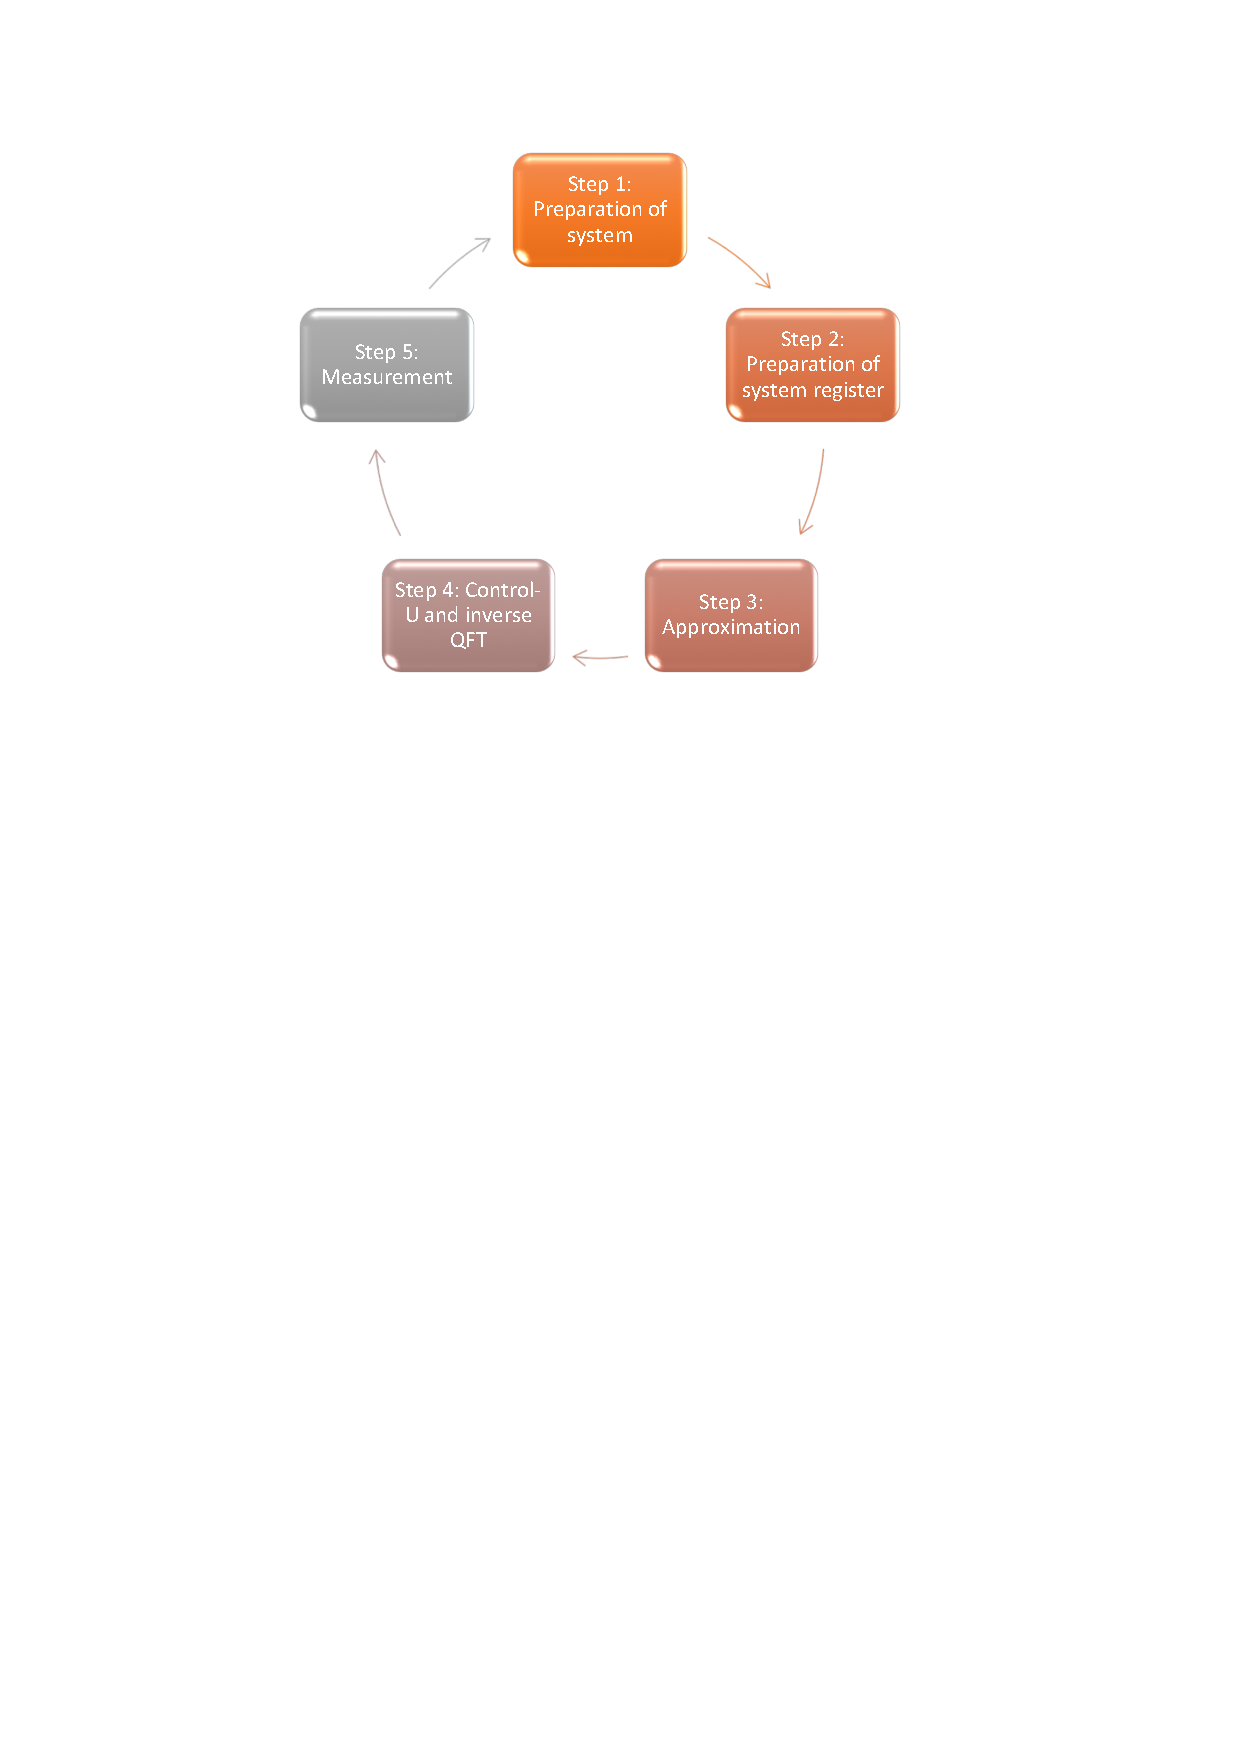
\includegraphics[width=15em]{PEA.pdf}
    \caption{PEA}
  \end{minipage}
  \end{center}

   
\end{figure}



\section*{Conclusion and Outlook}



\begin{figure}[H]
  \begin{center}
  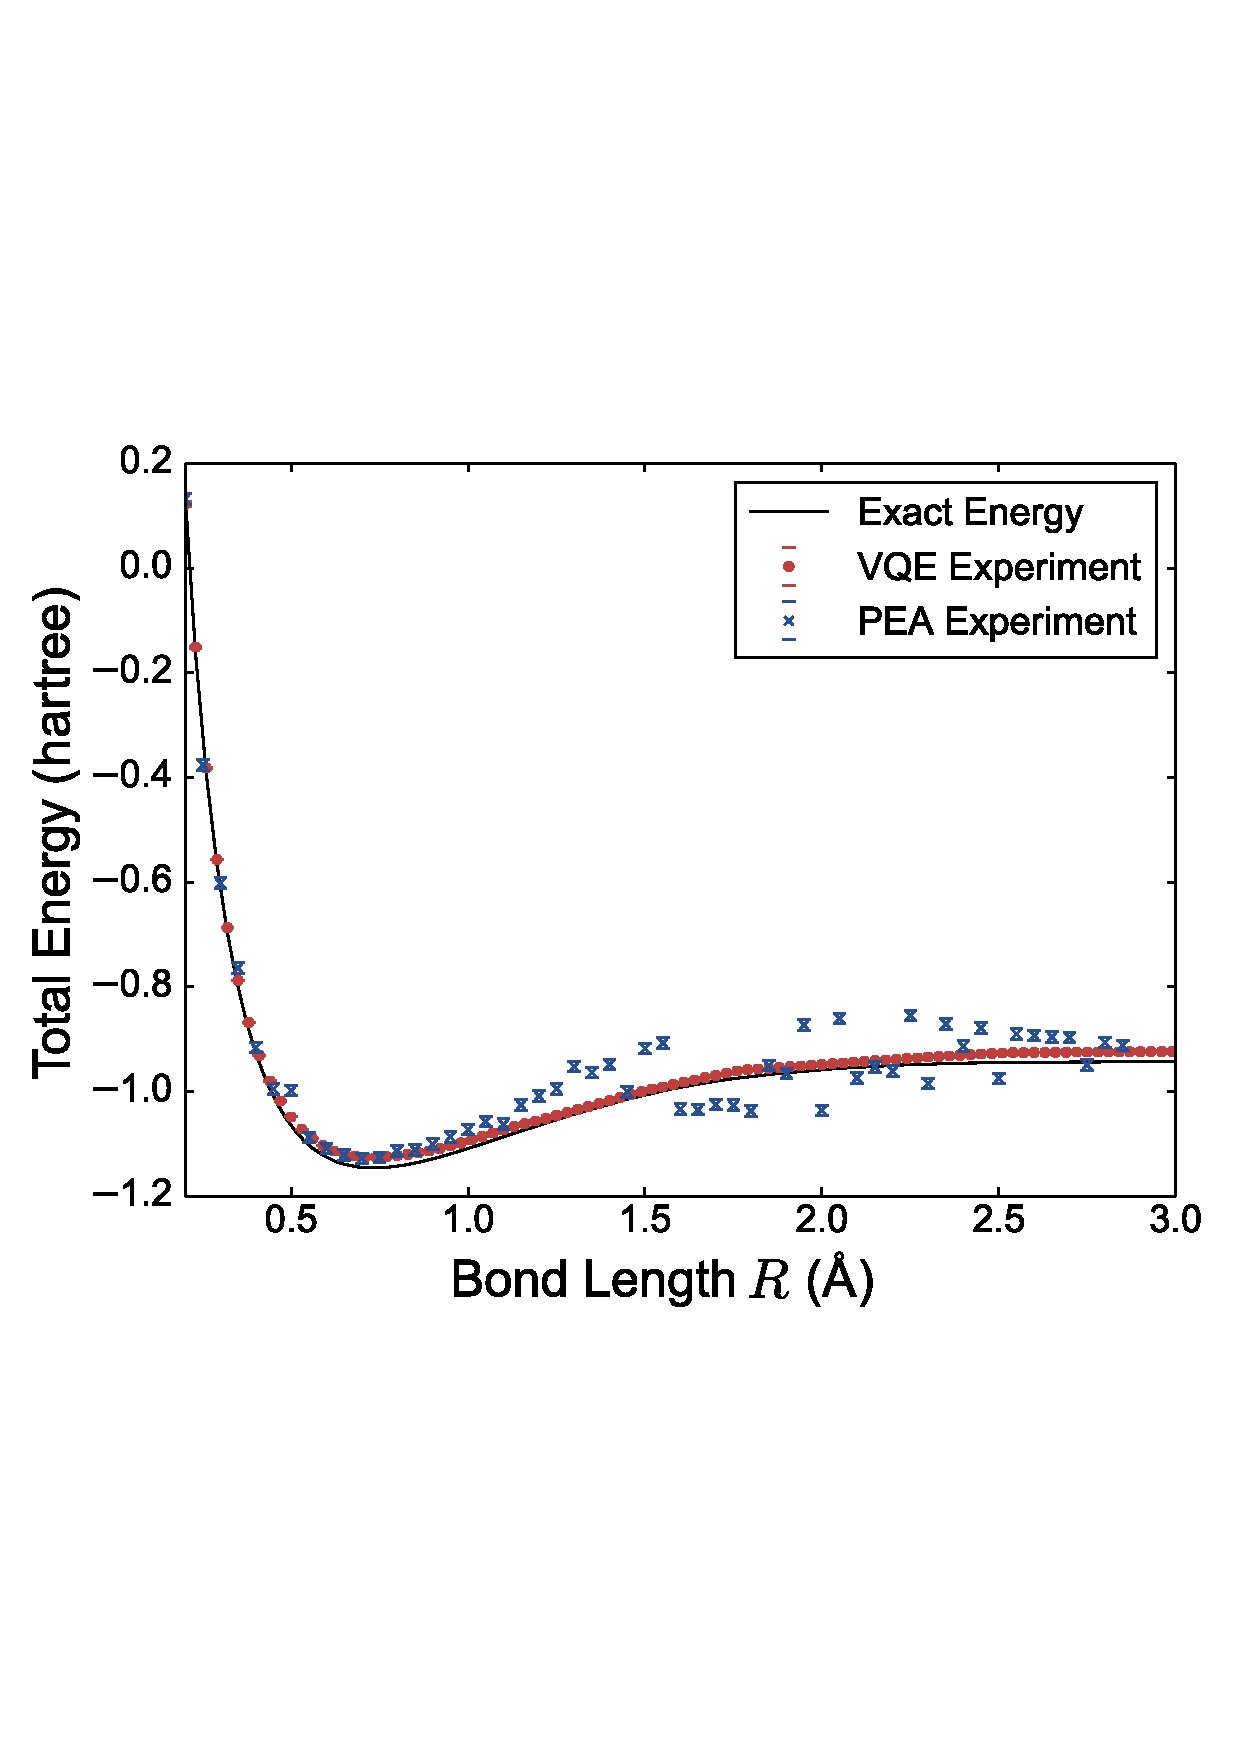
\includegraphics[scale=1.5]{result.pdf}
  \caption{Computed $H_2$ energy curve, energy surface of molecular hydrogen as determined by both VQE and PEA}
  \end{center}
    
 

   
\end{figure}

VQE was proven to work better than PEA because it gives more accurate results. Therefore, it is used more than PEA. Creating more algorithms such as VQE can lead to making new medicines, materials and other cool applications!


\end{multicols}
	
\end{document}
